\section{Accounts and Enrolments}
\subsection{Overview}
The ability to create and manage accounts and enrollments of students, teachers and administrators is a key feature of any LMS. Without being able to create and manage individual accounts for each type of user, the system will be impractical for use in educational environments, and without being able to enroll into courses and topics, many other features of our Meta LMS will not be useful.

\subsection{UI/UX}
There are 4 main pages relating to accounts and enrollment:
\begin{itemize}
  \item Sign in and sign up;
  \item Viewing and editing account details;
  \item administrators enrolling students and creating course invite codes; and,
  \item Students self-enrolling.
\end{itemize}

\textbf{Sign in and sign up}
The sign in and sign up screens need to allow users to enter the necessary details to either sign in or sign up, while also being as accessible as possible. Many designs already exist for these components so it is a matter of utilizing the features of existing designs that support accessibility the most. These features include high contrast colors, large readable text, a clear page flow and sufficient text instructions.

\begin{figure}[h!]
  \centering
  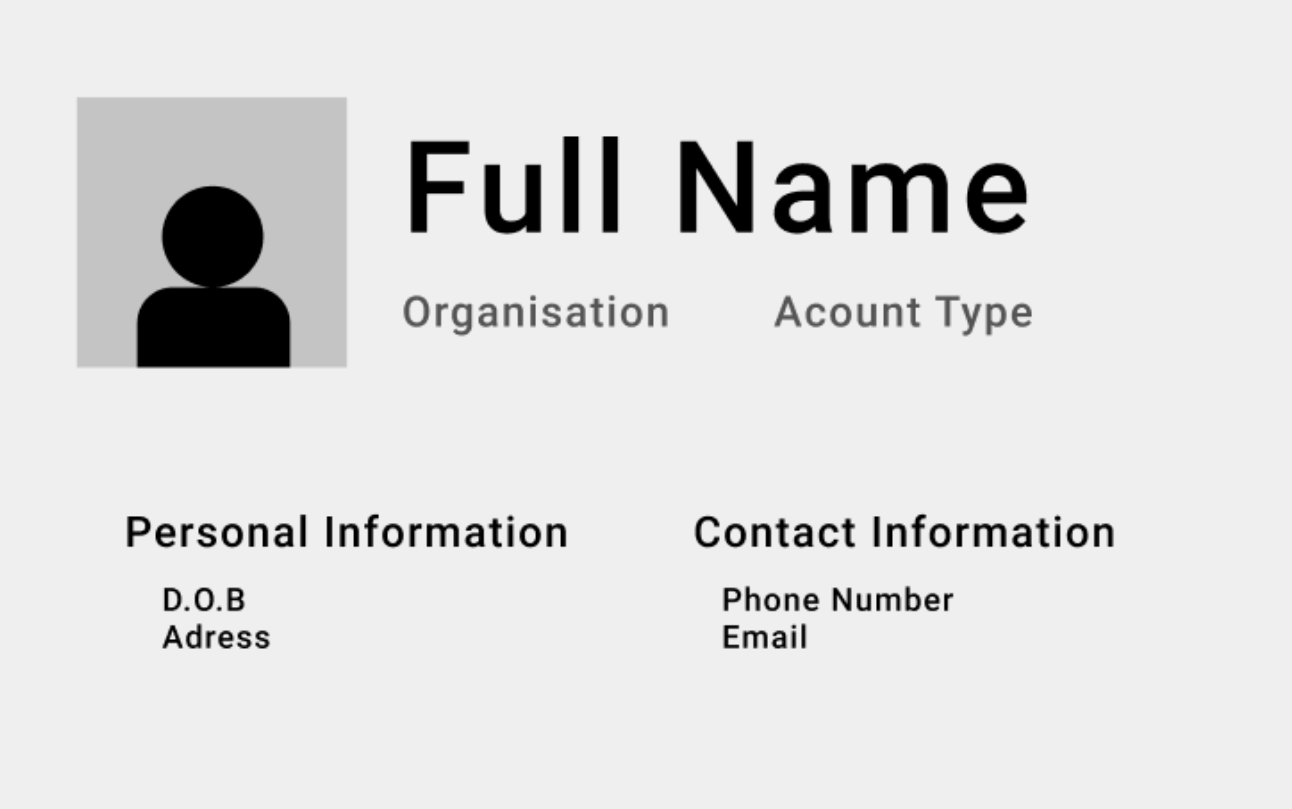
\includegraphics[scale=0.2]{images/accounts-profile}
  \caption{A user's view of their account.}
\end{figure}

\textbf{Viewing and Editing Account Details}
User's need to be able to easily view their account information, and that of other users. Accessibility is a key concern for this page, so a clear page flow and easy to read text are most important, as well as a sleek and visually appealing user interface to ensure that information can be comprehended from the page as easily as possible.

\begin{figure}[h!]
  \centering
  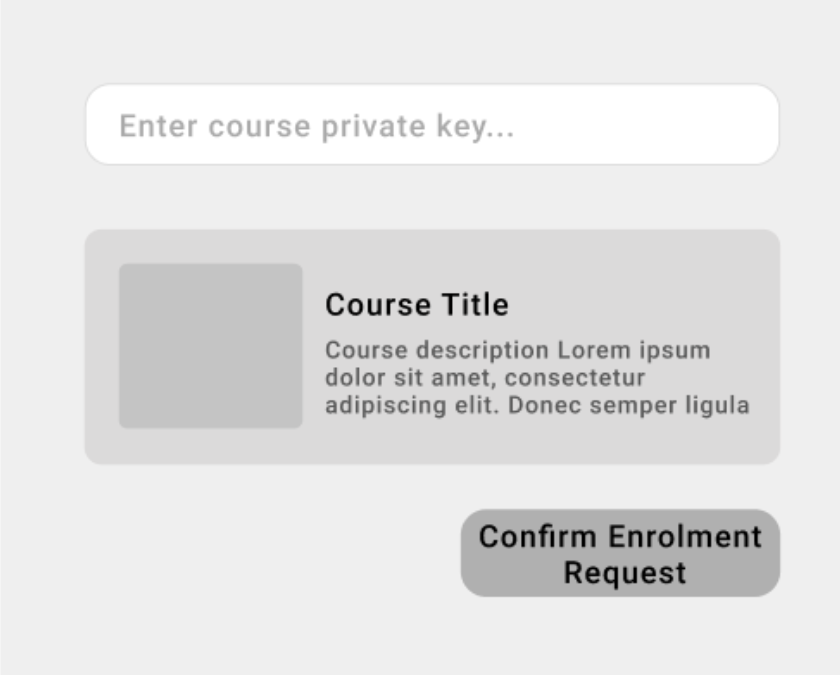
\includegraphics[scale=0.2]{images/accounts-code}
  \caption{A student user's screen to enrol in a course via invite code.}
\end{figure}

\textbf{Administrators Enrolling Students}
administrators need to be able to individually add student's to a course, and generate an invite code that students can use to enroll in a course. 

\begin{figure}[h!]
  \centering
  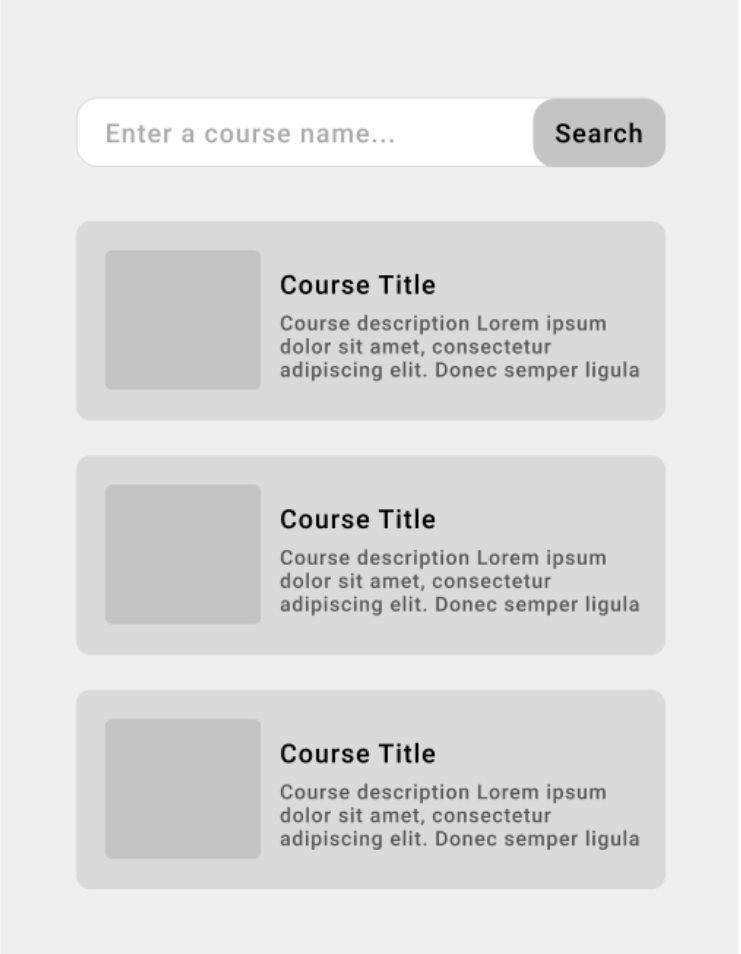
\includegraphics[scale=0.2]{images/accounts-search}
  \caption{A student user's view to search for courses and topics.}
\end{figure}

\textbf{Student's Self Enrolling}
A student user needs to be able to either enter a course invite code generated by an administrator, or search for a course or topic via its name or course code, to enroll themselves into a course. It is important that when searching for courses and topics, as much information is as clearly displayed as possible.

\subsection{Database}
The accounts system is also in charge of governing the data of the different users. Thus it is important to plan the design of the database schema for a user account. Below is an initial design of what the database table headings for a user may look like:

\begin{center}
    \begin{tabular}{|c|c|c|c|c|c|c|c|} 
        \hline
        id & type & name & email & password & phone & address & topics \\ [0.5ex] 
        \hline
    \end{tabular}
\end{center}

The ID field has dual purposes, it both stores a users student ID, and is also a unique identifier for every student. The type field stores the account type of a user, such as student or administrator. We also need to be able to store a users personal information, such as their name, phone number and address so there are fields for that. The user needs to be able to log in so an email and password will also be stored. Finally a list of all of the topics a user has completed must also be stored so that their progress can be reflected in any courses they are enrolled in.\\

This schema will likely change throughout Thesis B, as additional requirements for data to be attached to a user present themselves throughout development, but this design presents a starting point that covers a large portion of what will be the final representation of a user in the database.

\subsection{Requirements}
The initial requirements for the accounts and enrolment system are listed below, but are likely to change and become more specific throughout the following stages of the thesis. Each requirement has a priority that was measured by surveying the other thesis members. Higher priority items will be completed first, with medium and then low priority requirements to be implemented later in the project in their respective order.

\subsection{Functional Requirements}
\textbf{Accounts}
    \begin{enumerate}
    \item Users can register and login \textcolor{Red}{High}
    \item Users can view and update their details \textcolor{Red}{High}
    \item administrators can manage users, roles and permissions \textcolor{Red}{High}
    \item administrators can create accounts on behalf of students \textcolor{Orange}{Medium}
    \item administrators can view other users account details \textcolor{Orange}{Medium}
    \end{enumerate}

\textbf{Enrollments}
    \begin{enumerate}
    \item administrators can open and close enrolments for courses \textcolor{Red}{High}
    \item administrators can enrol and un-enroll students on their behalf \textcolor{Red}{High}
    \item administrators can generate course invite codes \textcolor{Red}{High}
    \item administrators can set courses to be open enrolment or invite/code only \textcolor{Orange}{Medium}
    \item Students can enrol themselves in courses with a code \textcolor{Red}{High}
    \item Students can enrol themselves in an open course or topic \textcolor{Red}{High}
    \item Students can search for open courses \textcolor{Blue}{Low}
    \end{enumerate}

\subsection{Timeline}

\begin{figure}[h!]
  \centering
  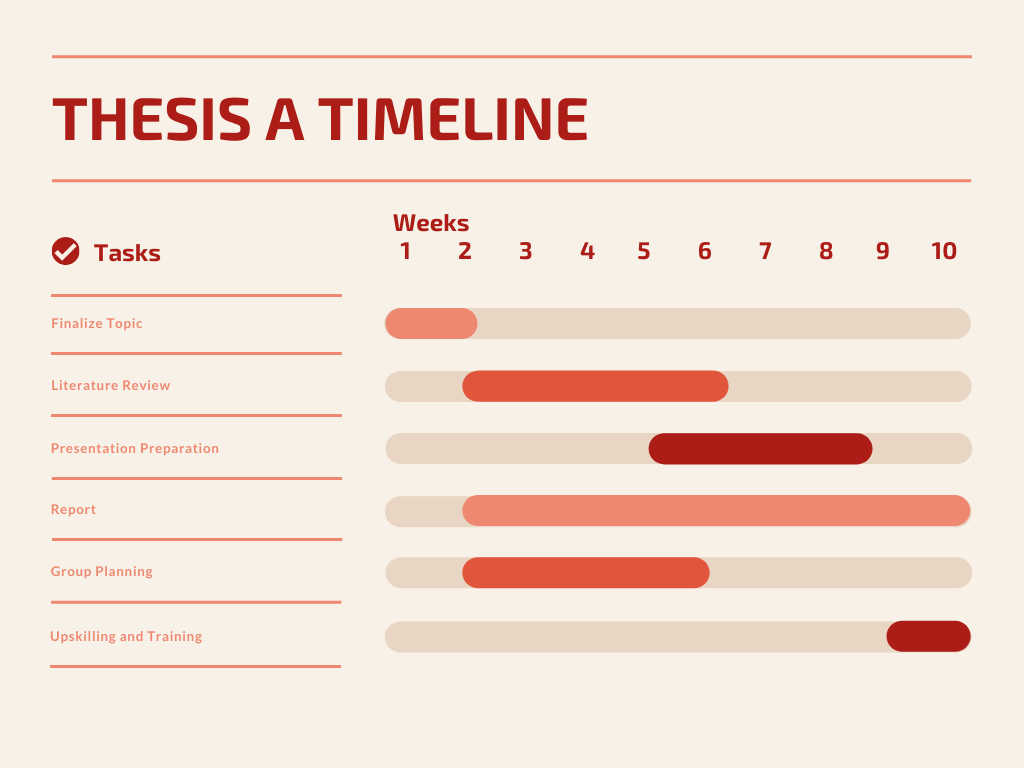
\includegraphics[scale=0.4]{accounts-thesis-a}
  \caption{Thesis A Timeline.}
\end{figure}
Thesis A primarily focused on assessing the state-of-the-art through the literature review, and creating a plan for Thesis B and C, while also preparing this initial report and the initial presentation. It was also necessary to collaborate among the group to evenly split the workload and agree on a vision of what the future of the project was to look like, as well as on technical details such as the software stack.

\begin{figure}[h!]
    \centering
    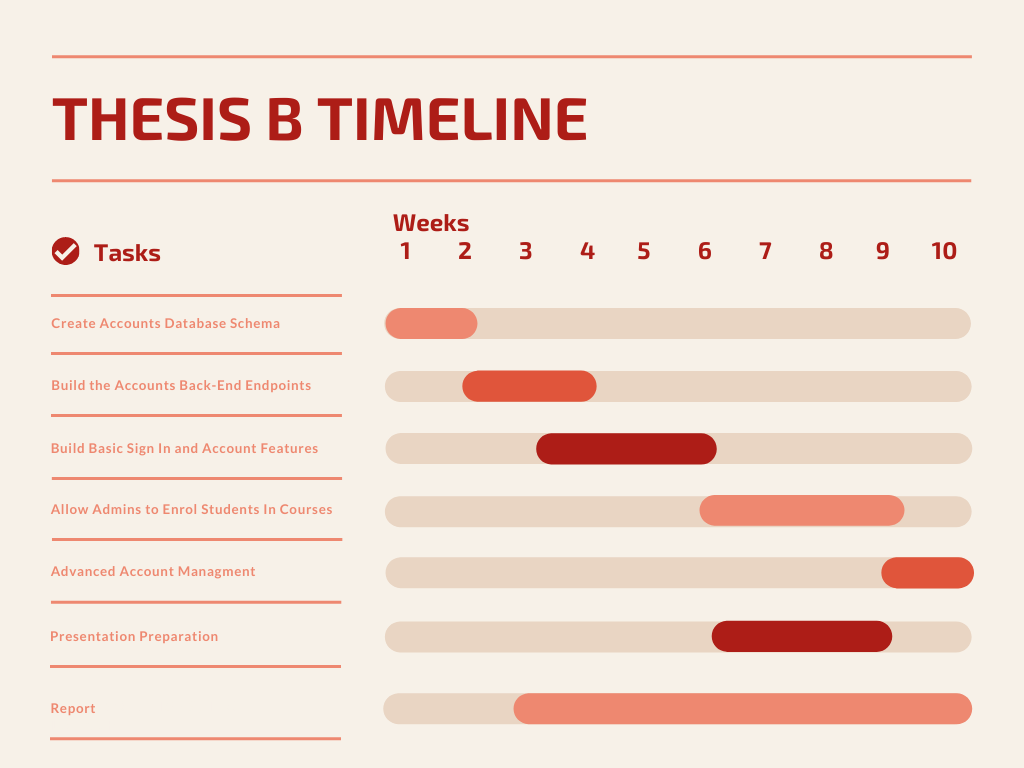
\includegraphics[scale=0.4]{accounts-thesis-b}
    \caption{Thesis B Timeline.}
\end{figure}
Thesis B's primary focus is to implement as much of the assessments and enrolments feature as possible, so that an adequate prototype can be demonstrated towards the end of term 2. During this time most of the core features of the accounts and enrolment systems will be implemented. It is important to implement the core of these features early, as many of the other features of our Meta LMS are dependent on the ability to create and manage user accounts.

\begin{figure}[h!]
    \centering
    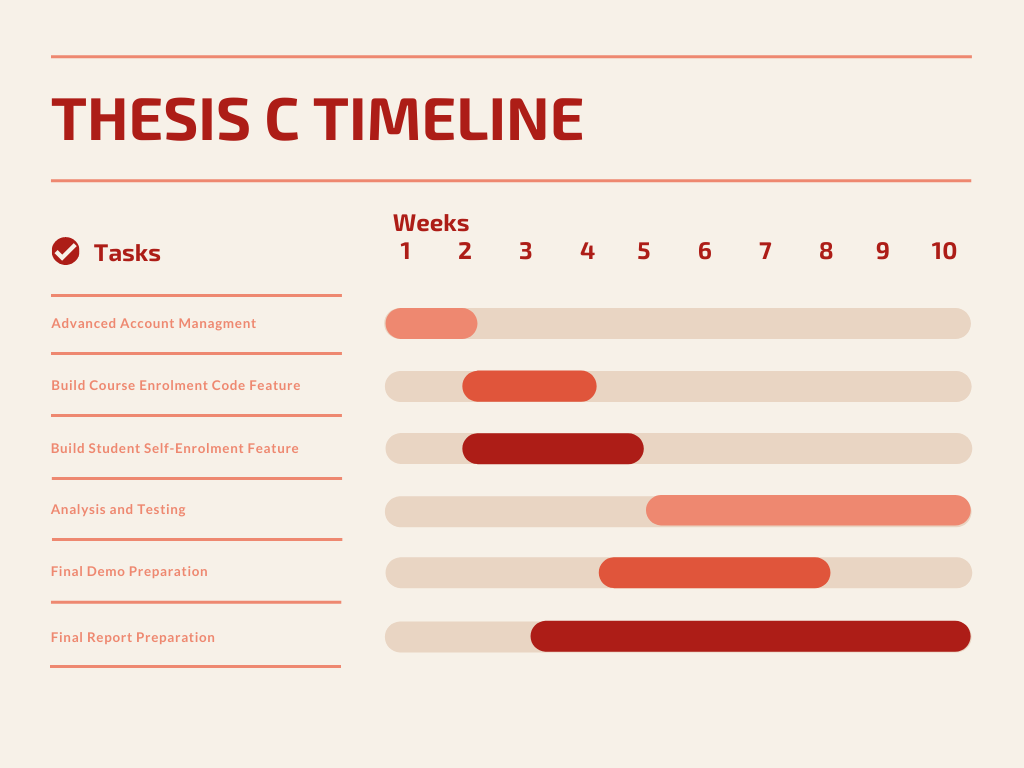
\includegraphics[scale=0.4]{accounts-thesis-c}
    \caption{Thesis C Timeline.}
\end{figure}
The goals of Thesis C are to finalize core features, add any extension features as time permits, and to test and polish these systems to ensure the best possible version of the project will be delivered. Thesis C is also when these systems will be analyzed and evaluated against the criteria to be specified below, to assess how well these features achieved their goals withing the Meta LMS.

\subsection{Milestones}
The major development milestones for the accounts and enrolments features are as follows:
    \begin{enumerate}
        \item Week 2 Term 2: Build the accounts database schema.
        \item Week 4 Term 2: Build the accounts back-end endpoints.
        \item Week 6 Term 2: Allow users to create an account, sign in, and view their account information.
        \item Week 9 Term 2: Allow administrators to enrol students into a course.
        \item Week 2 Term 3: Allow users to update their account information.
        \item Week 4 Term 3: Allow administrators to generate an enrolment code, allow students to enrol themselves in open courses.
        \item Weeks 5-11 Term 3: Analysis and Testing.
    \end{enumerate}

\subsection{Evaluation}
In addition to assessing how well the accounts and enrolments features meet the requirements specified above, it will also be evaluated on how well it meets the following criteria:
\begin{enumerate}
    \item Performance - Whether it is quick to create an account or sign-up, and the responsiveness of the enrolment features.
    \item Accessibility - Can a wide array of users easily navigate account management areas and enrolment forms.
    \item UI/UX - Are the features easy to use and attractive.
    \item Errors - Are the features bug and error free.
\end{enumerate}